% Auto-generated by generate_report.py — do not edit manually
% Preamble mirrors oxengthesis.cls so figures match the body text:
% Carlito as main font, Latin Modern Math via unicode-math.
\documentclass[border=6pt]{standalone}
\usepackage{fontspec}
\setmainfont{Carlito}
\usepackage{unicode-math}
\setmathfont{Latin Modern Math}
\usepackage{pgfplots}
\pgfplotsset{compat=1.18}
\usepgfplotslibrary{groupplots}
\usetikzlibrary{patterns,positioning}
\begin{document}
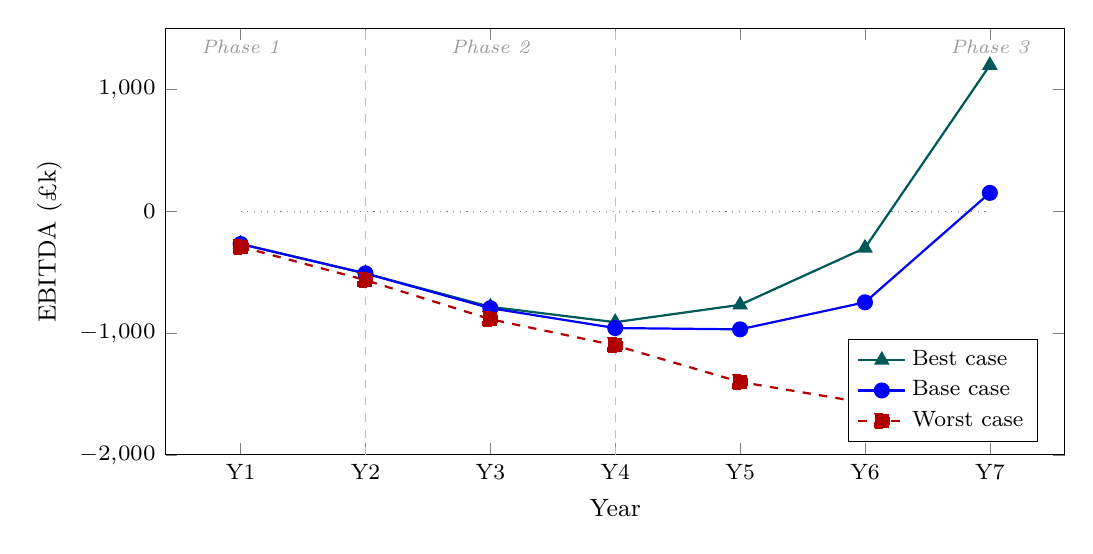
\begin{tikzpicture}
    \begin{axis}[
            width=13cm,
            height=7cm,
            xlabel={Year},
            symbolic x coords={Y1,Y2,Y3,Y4,Y5,Y6,Y7},
            xtick=data,
            legend style={
                font=\footnotesize,
                at={(0.02,0.98)},
                anchor=north west,
                legend cell align={left},
            },
            tick label style={font=\footnotesize},
            label style={font=\small},
        ylabel={EBITDA (\pounds k)},
        ymin=-2000, ymax=1500,
        legend pos=south east,
    ]
    \draw[dashed,gray!50] (axis cs:Y2,-2000) -- (axis cs:Y2,1500);
    \draw[dashed,gray!50] (axis cs:Y4,-2000) -- (axis cs:Y4,1500);
    \node[anchor=north,font=\scriptsize\itshape,gray!80] at (axis cs:Y1,1480) {Phase 1};
    \node[anchor=north,font=\scriptsize\itshape,gray!80] at (axis cs:Y3,1480) {Phase 2};
    \node[anchor=north,font=\scriptsize\itshape,gray!80] at (axis cs:Y7,1480) {Phase 3};
    \addplot[thick,teal!70!black,mark=triangle*,mark size=2.5pt] coordinates {(Y1,-270.1) (Y2,-511.6) (Y3,-785.5) (Y4,-911.6) (Y5,-769.0) (Y6,-302.7) (Y7,1195.9)};
    \addplot[thick,blue,mark=*,mark size=2.5pt] coordinates {(Y1,-270.1) (Y2,-511.6) (Y3,-796.7) (Y4,-959.6) (Y5,-970.3) (Y6,-748.4) (Y7,149.2)};
    \addplot[thick,red!70!black,mark=square*,mark size=2.5pt,dashed] coordinates {(Y1,-292.2) (Y2,-565.9) (Y3,-887.4) (Y4,-1101.9) (Y5,-1401.5) (Y6,-1572.9) (Y7,-1665.1)};
    \draw[dotted,gray,thin] (axis cs:Y1,0) -- (axis cs:Y7,0);
    \legend{Best case, Base case, Worst case}
    \end{axis}
\end{tikzpicture}

\end{document}
